Программный комплекс реализует предложенные этапы оцифровки книг (сегментации страницы на логические блоки, предобработка изображений, специализированных методов извлечения). Пример работы программы и промежуточные этапы приставлены на рис.~\ref{fig:example_prog}. Далее рассмотрим каждый этап подробнее.

\begin{figure*}[t]
	\centering
	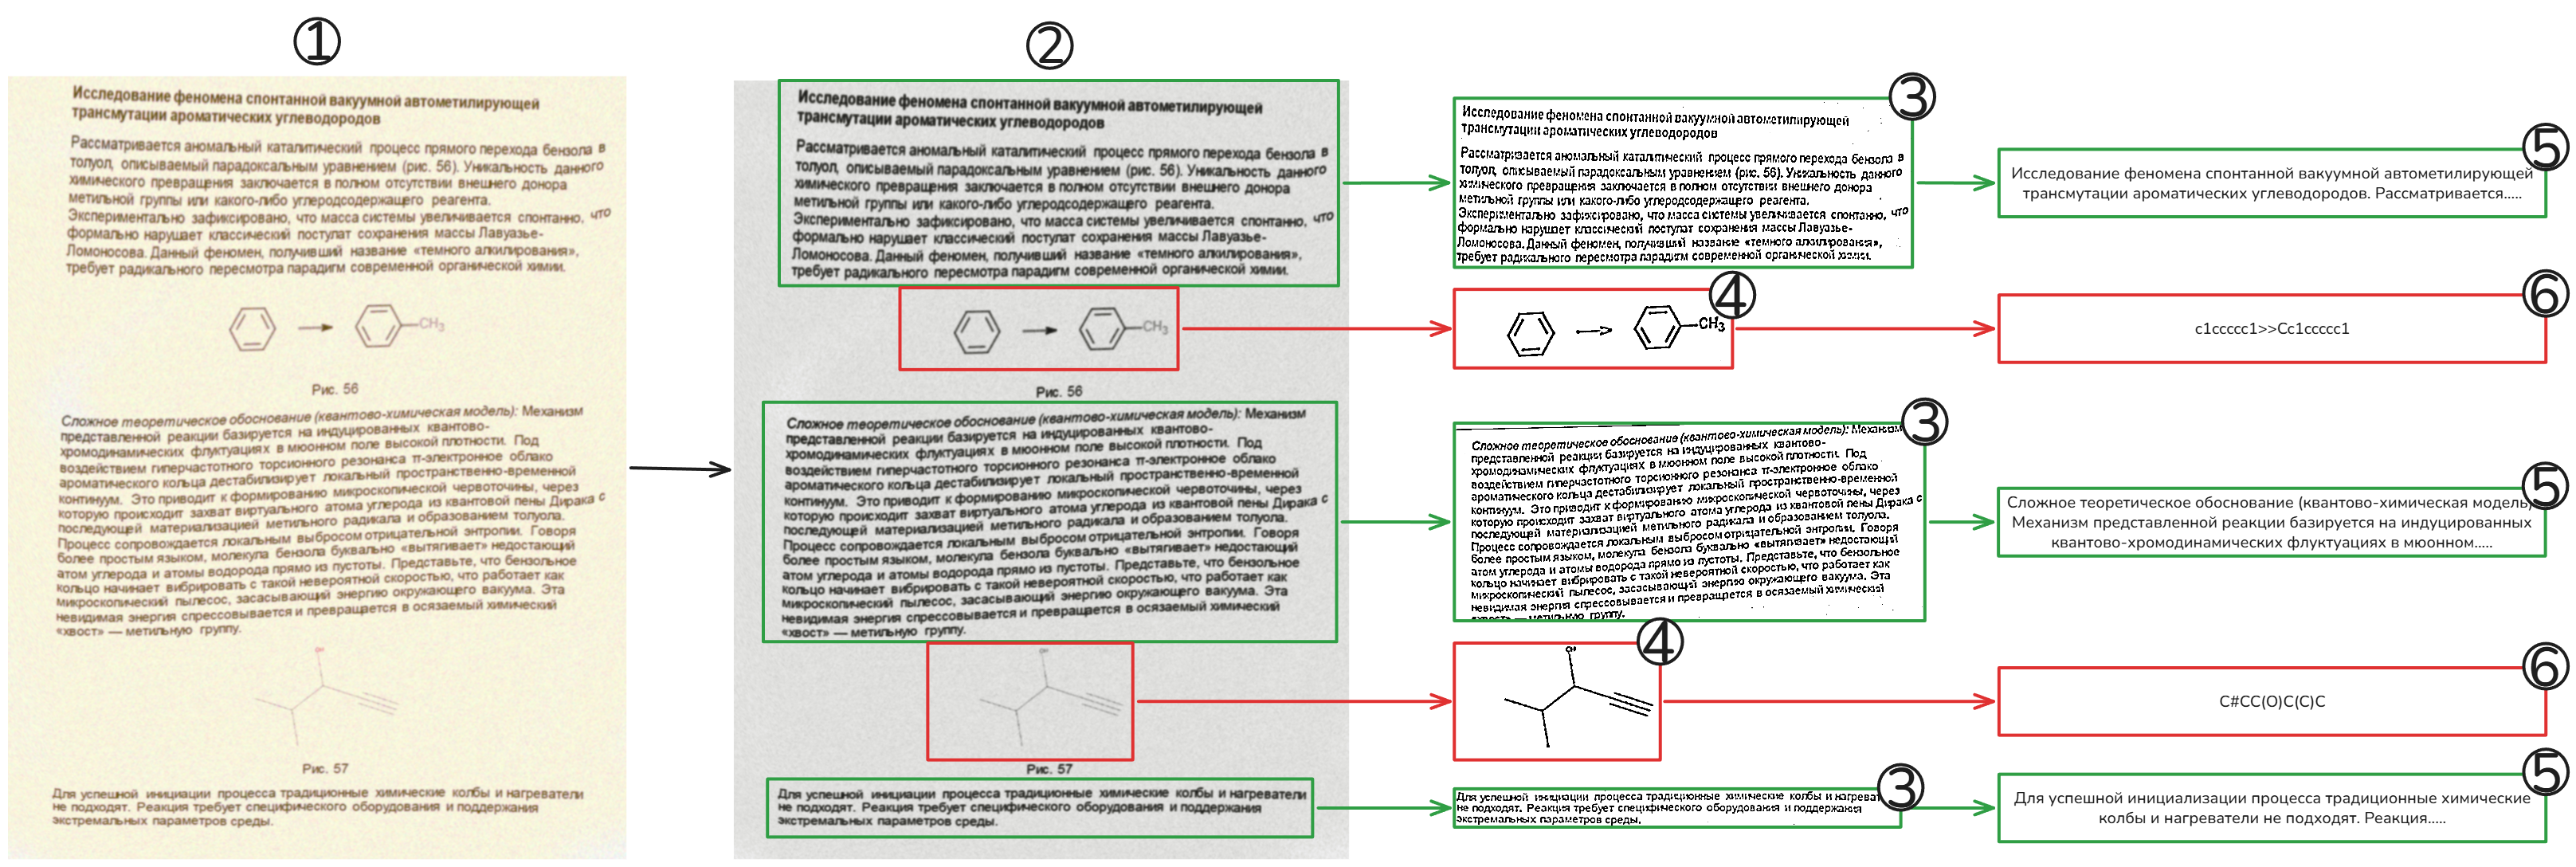
\includegraphics[width=1\linewidth]{img/example_prog.png}
	\bicaption
	{Пример работы программы: \textit{1} -- исходная страница; \textit{2} -- результат работы сегментатора; \textit{3} -- предобработанный текст страницы; \textit{4} -- предобработанная формула; \textit{5} -- машино-обрабатываемый текст; \textit{6} -- формула в формате <<SMILES>>}
	{Example of the program's operation: \textit{1} -- source page; \textit{2} -- segmenter's result; \textit{3} -- preprocessed page text; \textit{4} -- preprocessed formula; \textit{5} -- machine-processed text; \textit{6} -- formula in <<SMILES>> format}
	\label{fig:example_prog}
\end{figure*}

